\apendice{Estudio experimental}

Este apartado está dedicado a describir las diferentes pruebas realizadas a lo largo de la elaboración del proyecto para demostrar su funcionalidad. 

\section{Cuaderno de trabajo}

El desarrollo experimental del proyecto lo podemos dividir en dos bloques: pruebas con el relé y la mini bomba y pruebas con el sensor. Estas pruebas se han realizado para verificar que todos los componentes funcionan de forma adecuada.

\subsection{Relé}
Para probar que el relé y la mini bomba funcionan correctamente, he desarrollado un código basado en la activación del relé para encender y apagar la bomba. Para ello el primer paso es realizar las conexiones tal y como se explica en el \textit{Anexo B} en la Figura \ref{fig:conex_rele}. Una vez hecho, introduciremos la mini bomba en un recipiente con agua y conectaremos una manguera que vaya de la mini bomba a otro recipiente vacío para echar el agua. Esto lo podemos observar en la Figura \ref{fig:conex_rele_bomba}.
\begin{figure}[H]
    \centering
    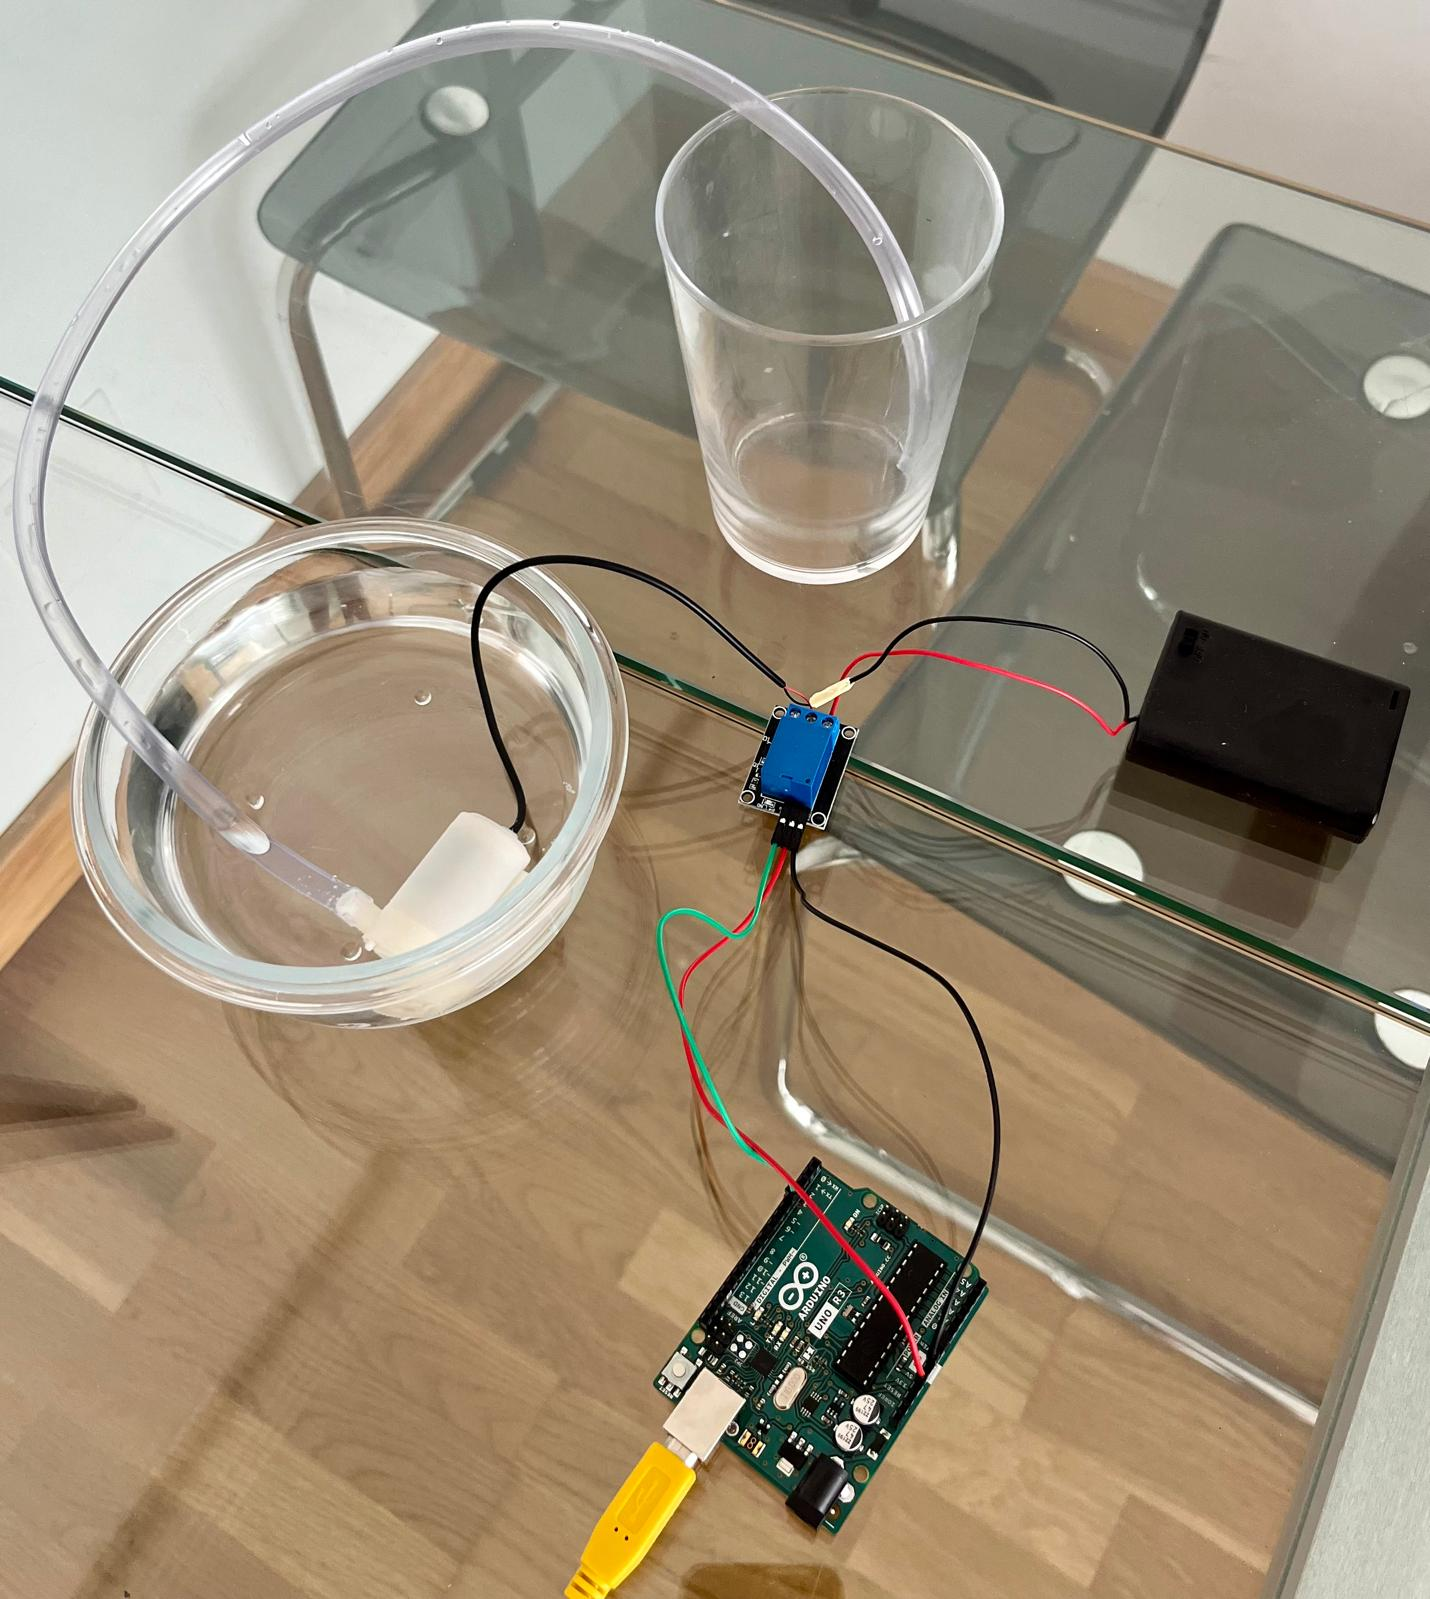
\includegraphics[width=0.7\textwidth]{img/releBomba.jpg}
    \caption{Conexión relé y mini bomba con tanques de agua. Imagen propia}
    \label{fig:conex_rele_bomba}
\end{figure}


El código desarrollado es el siguiente:

\begin{lstlisting}
const int rele = 4; // El rele esta conectado al pin digital 4
int contador = 0; // Contador para limitar el numero de veces que el rele se activa para encender la mini bomba
bool pruebaCompletada = false; // Variable booleana inicializada a false para controlar cuando la prueba ha finalizado

void setup() {
  Serial.begin(9600);
  pinMode(rele, OUTPUT); // Configuracion del rele como salida
  digitalWrite(rele, LOW); // Inicialmente el rele esta apagado
}

void loop() {
  if (!pruebaCompletada && contador < 2) { 

    // ACTIVAR MINI BOMBA
    Serial.println("Activando la mini bomba...");
    digitalWrite(rele, HIGH); // Activa el rele para encender la bomba durante 1,5 seg
    delay(1500); 
    
    // DESACTIVAR MINI BOMBA
    Serial.println("Bomba desactivada");
    digitalWrite(rele, LOW); // Desactiva el rele para apagar la bomba
    delay(3000);
    
    contador++;
     
  } else if (!pruebaCompletada) {
    Serial.println("Prueba completada"); 
    pruebaCompletada = true; // La prueba ha sido completada
    delay(1000); 
    return; 
  }
}
\end{lstlisting}

En el Repositorio, dentro de la carpeta Arduino, podemos encontrar el documento \textit{rele.ino}, que contiene el código anterior, mientras que en la carpeta demostraciones podemos encontrar un vídeo \textit{rele.mp4} demostrando que funciona correctamente.

\subsection{Sensor de presión NPX MPX5010DP}
Al igual que con el relé, se han realizado pruebas con el sensor para demostrar su funcionalidad. Para ello necesitamos realizar las conexiones de forma adecuada, tal y como indica la Figura \ref{fig:conex_sens} y poner la manguera en el sensor para crear un colchón de aire, ya que como hemos mencionado en apartados anteriores, este sensor no es sumergible. Esta manguera la hemos pegado con silicona a un recipiente, al cual iremos añadiendo agua para aumentar la presión. Lo podemos observar en la Figura \ref{fig:conex_sen_tanq}.
\begin{figure}[h]
    \centering
    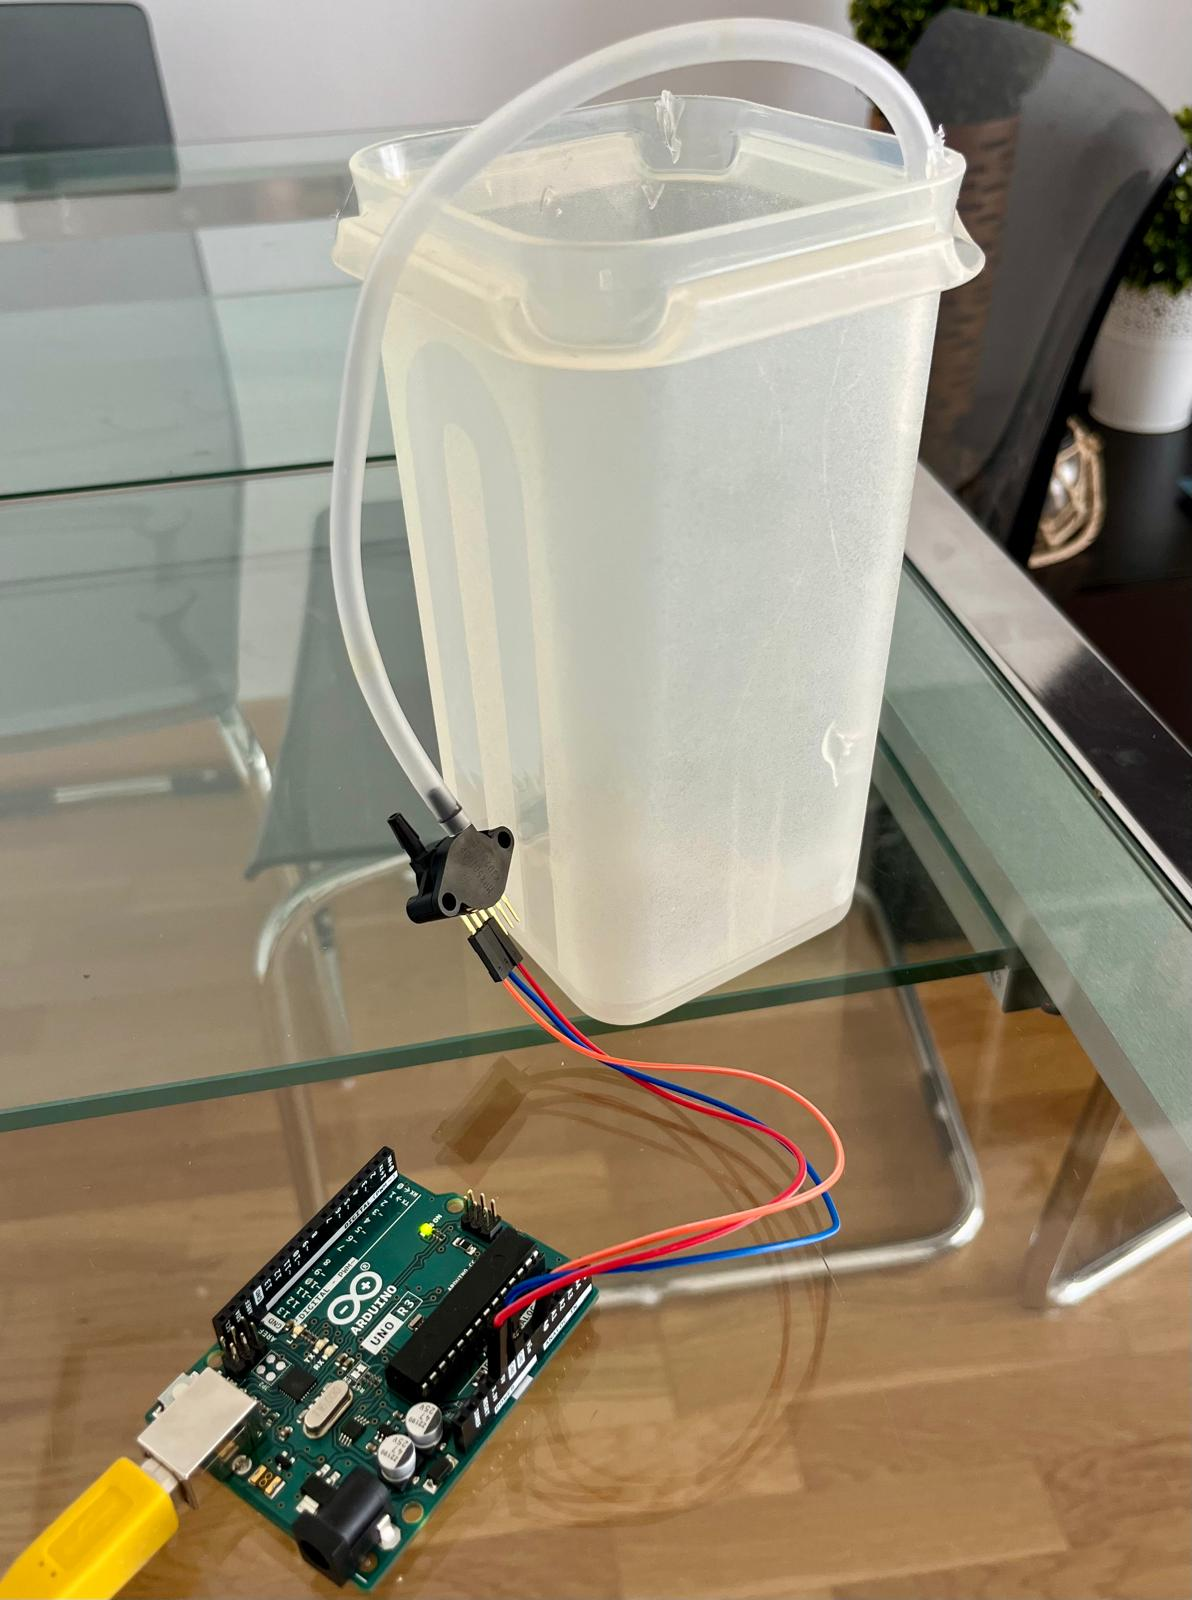
\includegraphics[width=0.6\textwidth]{img/sensortanque.jpg}
    \caption{Conexión del sensor con tanque de agua. Imagen propia}
    \label{fig:conex_sen_tanq}
\end{figure}

Cuando conectamos la placa de Arduino al ordenador y compilamos el programa, el sensor hace lecturas negativas de -0.56 mmHg \footnote{Este valor no siempre es ese, puede variar y hay que calibrarlo al inicio de cada uso.}, cuando debería de dar 0.00 mmHg ya que el recipiente está vacío. Para solucionarlo basta con sumar +0.56 al valor final de presión, para que así las lecturas con el tanque vacío sean de 0.00 mmHg. Lo podemos observar en las Figuras \ref{fig:lect-neg}, \ref{fig:tol} y \ref{fig:lectcero}.
\begin{figure}[H]
    \centering
    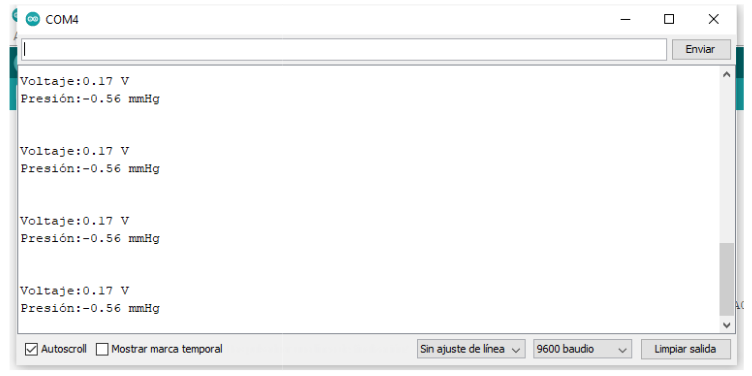
\includegraphics[width=1\textwidth]{img/lecturasnegativas.PNG}
    \caption{Lecturas negativas del sensor. Imagen propia}
    \label{fig:lect-neg}
\end{figure}

\begin{figure}[H]
    \centering
    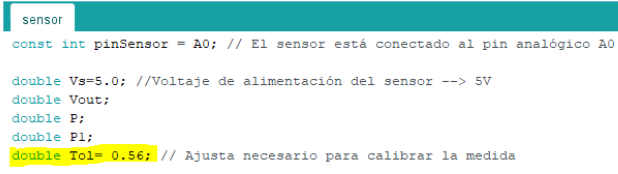
\includegraphics[width=1\textwidth]{img/tol.PNG}
    \caption{Tolerancia. Imagen propia}
    \label{fig:tol}
\end{figure}

\begin{figure}[H]
    \centering
    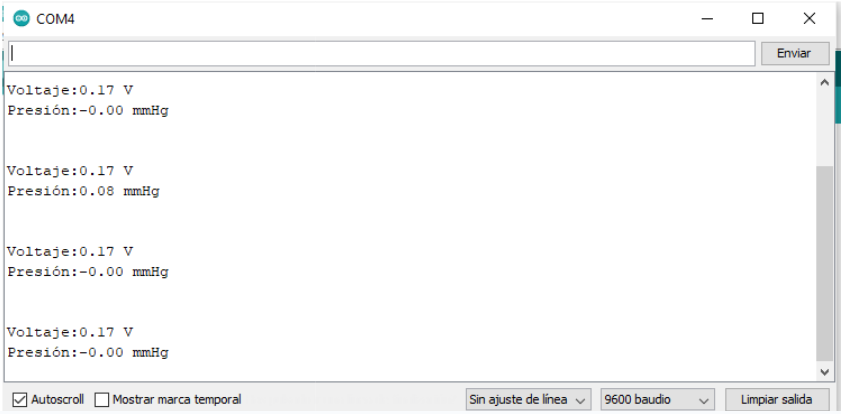
\includegraphics[width=1\textwidth]{img/lectcero.PNG}
    \caption{Sensor calibrado, lecturas iniciales correctas. Imagen propia}
    \label{fig:lectcero}
\end{figure}

Una vez calibrado, comenzamos a echar agua para que la presión aumente. Esto lo podemos ver en el vídeo \textit{sensor.mp4} contenido en la carpeta demostraciones del Repositorio. También podemos encontrar el documento \textit{sensor.ino}, que contiene el siguiente código.

\begin{lstlisting}
const int pinSensor = A0; // El sensor esta conectado al pin analogico A0

double Vs=5.0; //Voltaje de alimentacion del sensor --> 5V
double Vout;
double P; 
double P1;
double Tol= 0.56; // Ajusta necesario para calibrar la medida


void setup()
{
  Serial.begin(9600);
  
}
void loop() {
    
    Vout = float(analogRead(pinSensor))*5.0/1023.; //Lectura del voltaje con analogRead() --> Leemos lo que hay en el pin A0 (V)
  
    P = (Vout-0.04*Vs) / (0.09*Vs); //Calculamos la presion (Figura 4 datasheet)kPa
    P1 = P*7.50062+Tol; //P1 es la presion en mmHg 1kPa = 7.50062mmHg 
    
    Serial.print("\n\nVoltaje:");
    Serial.print(Vout);
    Serial.println(" V");
    Serial.print("Presion:");
    Serial.print(P1);
    Serial.println(" mmHg");
  
    delay(5000);
    
  }
\end{lstlisting}

\section{Observaciones}
En este proyecto se ha empleado la presión hidrostática\footnote{La presión hidrostática es la presión a la que está sometido un cuerpo sumergido en un fluido, debido a la columna de líquido que tiene sobre él \cite{presionhidro}.} del agua, cuya fórmula es la siguiente: 
\[
P = \rho g h
\]

donde:
\begin{itemize}
    \item \( P \): presión hidrostática,
    \item \( \rho \): densidad del agua,
    \item \( g \): fuerza de gravedad,
    \item \( h \): altura de la columna de agua.
\end{itemize}

La presión ha ido aumentando a medida que se echaba más agua al tanque, es decir, con la altura, ya que la gravedad y la densidad del agua han permanecido constantes en todo momento.